% ─────────────────────────────────────────────────────────────────────────────
% LiDAR Point Cloud Denoising for Autonomous Driving Applications
% Capstone Project Proposal — CPG No. 5, TIET Patiala
%
% Recreated LaTeX source (the original .tex was unavailable; this file was
% reconstructed faithfully from capstone_edited (7).pdf, March 2026 build).
%
% FIXES relative to the original PDF:
%   * Need Analysis: two broken citations [?, ?] on the adversarial-attack
%     claim now cite new references [11] (Cao et al., CCS 2019) and
%     [12] (Sun et al., USENIX Security 2020).
%   * Need Analysis: broken [?] on the SOR global-threshold limitation now
%     cites the denoising survey [5].
%   * Section 3.1: broken [?] on SOR over-smoothing now cites Heinzler et
%     al. [6], who benchmarked SOR/ROR failure modes in adverse weather.
%   * TODO(team): the cover page previously said "Siddant Singh" while the
%     roles table said "Siddhant Singh". Pending confirmation, the roles
%     table Name column is left blank (roll numbers retained).
% ─────────────────────────────────────────────────────────────────────────────
\documentclass[12pt,a4paper]{article}

\usepackage[a4paper,margin=1in,bottom=1.2in]{geometry}
\usepackage{graphicx}
\usepackage{amsmath,amssymb}
\usepackage{booktabs}
\usepackage{array}
\usepackage{setspace}
\usepackage{tikz}
\usetikzlibrary{shapes.geometric, arrows.meta, positioning}
\usepackage{fancyhdr}
\usepackage{lastpage}
\usepackage{caption}
\usepackage[colorlinks=true, linkcolor=red, citecolor=green!60!black]{hyperref}

\setstretch{1.35}
\setlength{\parindent}{0pt}
\setlength{\parskip}{8pt}

% "N of 15" page footer, as in the original document
\pagestyle{fancy}
\fancyhf{}
\renewcommand{\headrulewidth}{0pt}
\fancyfoot[C]{\thepage\ of \pageref{LastPage}}

\begin{document}

% ═══════════════════════ Title page ═══════════════════════
\begin{titlepage}
\begin{center}
\vspace*{1cm}
{\LARGE\bfseries LiDAR Point Cloud Denoising for\\Autonomous Driving Applications\par}

\vspace{1.4cm}
{\Large\bfseries Capstone Project Proposal}\\[4pt]
Submitted by:

\vspace{0.8cm}
\begin{tabular}{r l}
\textbf{102315247} & \textbf{Jayantika}\\[2pt]
\textbf{102315219} & \textbf{Siddant Singh}\\[2pt]
\textbf{102303537} & \textbf{Krish Agarwal}\\[2pt]
\textbf{102303703} & \textbf{Shardool Dhodawat}\\[2pt]
\textbf{102303640} & \textbf{Ramyak Sharma}\\
\end{tabular}

\vspace{0.8cm}
BE Third Year - COE/CSE \quad CPG No.~5

\vspace{1cm}
Under the Mentorship of\\[2pt]
{\large\bfseries Dr.~Lovi Dhamija}\\
Assistant Professor

\vspace{0.8cm}
% TIET logo — drop tiet_logo.png next to this file to include it
\IfFileExists{tiet_logo.png}{\includegraphics[height=2.4cm]{tiet_logo.png}}{\vspace{2.4cm}}

\vfill
{\large\bfseries Department of Computer Science and Engineering\\[4pt]
Thapar Institute of Engineering and Technology, Patiala}\\[10pt]
{\bfseries March, 2026}
\end{center}
\end{titlepage}

% ═══════════════════════ Contents ═══════════════════════
\pagenumbering{roman}          % front matter: distinct numbering keeps
\setcounter{page}{2}           % hyperref page anchors unique
\thispagestyle{empty}
\tableofcontents
\clearpage

\pagenumbering{arabic}
\setcounter{page}{1}

% ═══════════════════════ Mentor Consent Form ═══════════════════════
\section*{Mentor Consent Form}
\addcontentsline{toc}{section}{Mentor Consent Form}

I hereby agree to be the mentor of the following Capstone Project Team.

\textbf{Project Title:} LiDAR Point Cloud Denoising for Autonomous Driving Applications

\vspace{0.5cm}
\begin{center}
\renewcommand{\arraystretch}{2.2}
\begin{tabular}{|p{2cm}|p{6cm}|p{4.5cm}|}
\hline
\textbf{Roll No.} & \textbf{Name} & \textbf{Signature}\\\hline
 & & \\\hline
 & & \\\hline
 & & \\\hline
 & & \\\hline
 & & \\\hline
\end{tabular}
\end{center}

\vspace{1cm}
\textbf{NAME of Mentor:} \dotfill

\textbf{SIGNATURE of Mentor:} \dotfill

\textbf{NAME of Co-Mentor (if any):} \dotfill

\textbf{SIGNATURE of Co-Mentor:} \dotfill
\clearpage

% ═══════════════════════ 1. Project Overview ═══════════════════════
\section{Project Overview}

LiDAR (Light Detection and Ranging) sensors are widely used in autonomous
driving, robotics, and smart surveillance systems to capture accurate 3D
representations of the environment. However, raw LiDAR point cloud data is
often corrupted by noise due to environmental factors such as rain, fog,
dust, and sensor inaccuracies. This noise affects downstream tasks such as
object detection, localization, and scene understanding.

The proposed capstone project focuses on designing a robust pipeline for
denoising LiDAR point clouds. The system will be evaluated using standard
benchmark datasets such as KITTI, nuScenes, and Waymo Open Dataset, which
represent real-world driving and urban scenarios. The objective is to remove
noise while preserving important geometric and structural information of
objects.

The proposed solution aims to balance accuracy and computational efficiency,
enabling its application in near real-time settings. Such a system is crucial
for time-sensitive applications like autonomous vehicles and robotic
navigation, where reliable perception of the environment is essential for
safe and effective operation.
\clearpage

% ═══════════════════════ 2. Need Analysis ═══════════════════════
\section{Need Analysis}

The rapid growth of autonomous systems - including self-driving vehicles,
UAVs, and service robots - has significantly increased reliance on
LiDAR-based perception. These systems depend on accurate 3D point cloud data
to perform critical tasks such as obstacle detection, path planning, and
environment mapping. LiDAR has become the sensor of choice for Level 3 and
Level 4 autonomy, as no other single sensor provides the dense,
range-accurate 3D point cloud that collision avoidance and path planning
require.

Real-world LiDAR data is, however, consistently corrupted by noise arising
from three distinct sources. \emph{Environmental conditions} such as rain,
fog, and dust cause laser pulses to backscatter off suspended particles
before reaching their intended targets, generating spurious phantom points at
incorrect distances. \emph{Hardware limitations} - including multi-echo
interference between co-mounted sensors, intensity calibration errors, and
vibration-induced jitter - introduce systematic outliers that geometric
filters struggle to distinguish from valid returns. \emph{Motion artefacts}
arise because a spinning LiDAR takes approximately 100~ms to complete one
scan; at highway speeds, this displacement distorts the shape of nearby
objects along the direction of travel.

The downstream consequences are serious. Object detectors trained on clean
data degrade significantly on noisy inputs, ICP-based localisation diverges
in the presence of outliers, and SLAM pipelines can fail entirely under heavy
environmental noise. The sensitivity of deep 3D perception models to
point-level data quality is further underscored by the adversarial attack
literature: research has shown that even imperceptible, deliberately crafted
perturbations added to LiDAR point clouds are sufficient to cause
state-of-the-art detectors to fail catastrophically across multiple
architectures \cite{cao2019adversarial, sun2020towards}. If deliberate
micro-perturbations can break detectors so reliably, naturally occurring
noise - which is orders of magnitude less controlled - poses an equally
serious threat to perception reliability. Existing remedies fall into two
families, neither of which is fully satisfactory. Statistical filters (SOR,
ROR) are fast but apply a global threshold that erodes fine geometric detail
and cannot distinguish structure from noise semantically \cite{wang2025survey}.
Deep learning methods are more accurate but require GPU resources, large
labelled datasets, and often fail to generalise across weather types or
sensor configurations \cite{heinzler2020cnn}. A solution that is
simultaneously accurate, computationally efficient, and generalisable remains
an open problem - and is precisely the gap this project aims to address.
\clearpage

% ═══════════════════════ 3. Literature Survey ═══════════════════════
\section{Literature Survey}

LiDAR point cloud denoising has been an active research area for over a
decade, driven by the growing deployment of autonomous systems in
uncontrolled outdoor environments. The literature can be broadly organised
into four generations of approaches: classical statistical filters,
projection-based convolutional methods, native 3D deep learning
architectures, and generative models. Each generation has addressed
limitations of the previous one, while introducing its own trade-offs between
accuracy, computational cost, and generalisability. This survey examines each
family in turn and contextualises their relevance to the proposed project.

\subsection{Classical Statistical and Geometric Methods}

The earliest and most widely deployed denoising techniques operate directly
on point neighbourhood statistics without any learned components. Statistical
Outlier Removal (SOR), introduced as part of the Point Cloud Library (PCL)
\cite{rusu2011pcl}, computes for each point the mean distance $\bar{d}$ to
its $k$ nearest neighbours and removes any point whose $\bar{d}$ exceeds
$\mu + \alpha\sigma$, where $\mu$ and $\sigma$ are the global mean and
standard deviation of all neighbourhood distances and $\alpha$ is a user-set
multiplier. Radius Outlier Removal (ROR) takes a complementary approach: a
point is removed if it has fewer than a minimum count of neighbours within a
fixed radius $r$. Both methods run in $\mathcal{O}(n \log n)$ time using a
k-d tree, making them practical even on embedded hardware.

Despite their efficiency, classical filters carry well-known failure modes.
Because SOR applies a single global threshold, it is unable to distinguish
genuine sparse returns - such as the few points returned by a distant
pedestrian or a low-reflectivity road sign - from sparse noise clusters.
Tuning $k$ and $\alpha$ for dense near-field noise simultaneously causes
over-smoothing of thin or distant structures \cite{heinzler2020cnn}.
Bilateral filtering and Moving Least Squares (MLS) surface reconstruction
offer improved geometric fidelity by weighting neighbour contributions by
spatial proximity or fitting local polynomials to the surface, but both
introduce significantly higher computational cost and assume locally smooth
geometry that does not hold at object boundaries or sharp edges.

The collective limitation of all classical approaches is their lack of
semantic awareness: they operate on geometry alone and have no mechanism to
distinguish a noisy but structurally meaningful region from a clean but
uninformative one.

\subsection{Projection-Based Convolutional Methods}

A natural bridge between classical signal processing and modern deep learning
is to project the irregular point cloud onto a regular 2D representation and
apply standard convolutional neural networks (CNNs). Range image projection
maps each 3D point to a pixel in a cylindrical panorama by encoding its
depth, height, and reflectance. This preserves neighbourhood structure and
allows reuse of mature 2D CNN architectures without modification.

Heinzler et al. \cite{heinzler2020cnn} proposed one of the first CNN-based
weather denoising pipelines operating on range images. Their model was
trained on a labelled dataset of LiDAR scans collected under controlled rain
and fog conditions, with each point annotated as \emph{clear} or
\emph{precipitation}. Using a U-Net-style encoder-decoder, the network
achieved substantially higher precision-recall for noise classification than
SOR or ROR on their proprietary benchmark. A key finding was that
convolutional features learned to exploit the spatial coherence of
precipitation clusters - something purely statistical filters cannot do.
However, the range image projection introduces an inherent artefact: points
that lie at the same azimuth and elevation but at different ranges are mapped
to the same pixel, causing occlusion losses. The cylindrical projection is
also specific to spinning LiDARs and does not generalise to solid-state or
MEMS-based sensors with irregular scan patterns.

\subsection{Native 3D Deep Learning Architectures}

The limitations of projection motivated architectures that operate directly
in 3D, treating the point cloud as an unordered set. PointNet
\cite{qi2017pointnet} was the foundational work in this space: it applied
independent multi-layer perceptrons (MLPs) to each point, followed by a
symmetric aggregation function (max-pooling) to produce a global feature
vector invariant to point permutation. While PointNet proved highly effective
for classification and part segmentation, its per-point processing is local
and does not capture fine neighbourhood geometry. PointNet++
\cite{qi2017pointnetpp} addressed this by introducing a hierarchical grouping
mechanism - farthest point sampling followed by ball-query neighbourhood
aggregation - that learns features at multiple spatial scales, substantially
improving performance on tasks requiring local geometric understanding such
as surface normal estimation and denoising.

Graph-based methods represent an alternative approach to capturing local
structure. DGCNN \cite{wang2019dgcnn} constructs a $k$-nearest-neighbour
graph in feature space at each layer and applies edge convolutions that
aggregate relative feature differences from neighbours, enabling the network
to adapt its receptive field dynamically as features evolve. Applied to
denoising, graph convolutions can distinguish noise clusters - which
typically form isolated subgraphs - from surface points that participate in
large, well-connected components.

Transformer architectures have more recently been applied to point clouds.
Point Transformer \cite{zhao2021point} replaces graph convolution with a
localised self-attention operator: for each point, attention weights are
computed over its $k$ nearest neighbours using relative positional encodings,
and the output is a weighted sum of neighbour features. This formulation is
permutation-invariant by construction, captures richer geometric context than
edge convolutions, and achieves state-of-the-art results on ModelNet40
classification and ShapeNet part segmentation. For outdoor denoising, the
challenge is computational: a full self-attention over $N \sim 100{,}000$
points requires $\mathcal{O}(N^2)$ memory, necessitating local windowing or
strided sampling strategies that introduce their own boundary artefacts.

Score-based denoising methods, inspired by the connection between Langevin
dynamics and score matching, train a network to estimate the gradient of the
log-density of the clean point distribution and iteratively move noisy points
toward regions of higher density. This approach achieves competitive results
on synthetic ShapeNet noise benchmarks but has not been demonstrated on
large-scale outdoor driving data.

\subsection{Generative and Diffusion-Based Models}

The most recent direction in point cloud denoising draws from generative
modelling. Denoising Diffusion Probabilistic Models (DDPMs) \cite{ho2020ddpm},
originally developed for image synthesis, define a forward process that
gradually adds Gaussian noise to data and a reverse process that learns to
undo it. This framework has been adapted to point clouds by operating on
point coordinates directly, demonstrating high-quality generation of clean
shapes from heavily corrupted inputs. The key advantage over discriminative
models is that the diffusion prior implicitly regularises geometry - the
reverse process can reconstruct plausible surface structure even in regions
with very few clean points.

However, diffusion models carry a fundamental inference-time cost: each
denoising step requires a full forward pass through a large neural network,
and competitive quality typically requires hundreds to thousands of steps.
Accelerated sampling strategies reduce this gap but per-frame latency of
several seconds on a GPU still renders these models incompatible with 10~Hz
real-time requirements. Real-time deployment of diffusion-based denoising
therefore remains an open research problem.

\subsection{Comparison and Research Gap}

Table~\ref{tab:comparison} summarises the key methods discussed above across
three axes relevant to the proposed project.

\begin{table}[h]
\centering
\caption{Comparison of LiDAR point cloud denoising methods.}
\label{tab:comparison}
\renewcommand{\arraystretch}{1.3}
\begin{tabular}{|p{4.2cm}|p{2.5cm}|p{2.6cm}|p{3.6cm}|}
\hline
\textbf{Method} & \textbf{Accuracy} & \textbf{Real-Time} & \textbf{Generalisation}\\\hline
SOR / ROR \cite{rusu2011pcl} & Low & Yes & High\\\hline
CNN (range image) \cite{heinzler2020cnn} & High & Yes (GPU) & Weather-specific\\\hline
PointNet++ \cite{qi2017pointnetpp} & High & Marginal & Moderate\\\hline
DGCNN \cite{wang2019dgcnn} & High & No & Moderate\\\hline
Point Transformer \cite{zhao2021point} & Very High & No & Moderate\\\hline
Diffusion Models \cite{ho2020ddpm} & Very High & No & High\\\hline
\end{tabular}
\end{table}

As the table makes clear, no single method simultaneously achieves high
accuracy, real-time throughput, and broad generalisability. Classical methods
are fast but inaccurate; deep learning methods are accurate but slow or
hardware-dependent; generative models offer the best geometric fidelity but
are orders of magnitude too slow for embedded deployment.

Three specific gaps emerge from this survey. First, there is no lightweight
architecture that has been rigorously evaluated on large-scale outdoor
driving data under multiple noise types simultaneously - most deep learning
work is benchmarked on synthetic ShapeNet objects, which have very different
geometric properties to sparse, rotating-LiDAR scans of road scenes. Second,
existing methods treat denoising in isolation: they optimise reconstruction
metrics such as Chamfer Distance without measuring whether improved point
cloud quality actually translates into better downstream object detection
accuracy, which is ultimately the metric that matters for autonomous driving.
Third, real-time feasibility is rarely reported under consistent hardware
constraints, making it difficult to compare methods fairly for deployment.

The proposed project targets precisely these gaps. By training and evaluating
on KITTI and nuScenes, benchmarking against both reconstruction metrics and
detection accuracy, and explicitly profiling throughput against the 10~Hz
automotive LiDAR constraint, this work addresses limitations that
individually motivated prior methods but have not yet been treated as a
unified design objective.
\clearpage

% ═══════════════════════ 4. Objectives ═══════════════════════
\section{Objectives}

The main objectives of the proposed project are:

\begin{enumerate}
\item To study the characteristics of noise in LiDAR point cloud datasets.
\item To design a framework for denoising LiDAR point cloud data while
      preserving geometric and structural information.
\item To evaluate the performance of the proposed approach using standard
      metrics such as reconstruction error (Chamfer Distance, Hausdorff
      Distance) and improvement in downstream object detection accuracy.
\item To optimise the proposed approach for near real-time processing, making
      it suitable for deployment in autonomous systems.
\end{enumerate}
\clearpage

% ═══════════════════════ 5. Methodology ═══════════════════════
\section{Methodology}

% non-floating so the flowchart stays with the section heading, as in the
% original document
\begin{center}
\resizebox{!}{0.78\textheight}{%
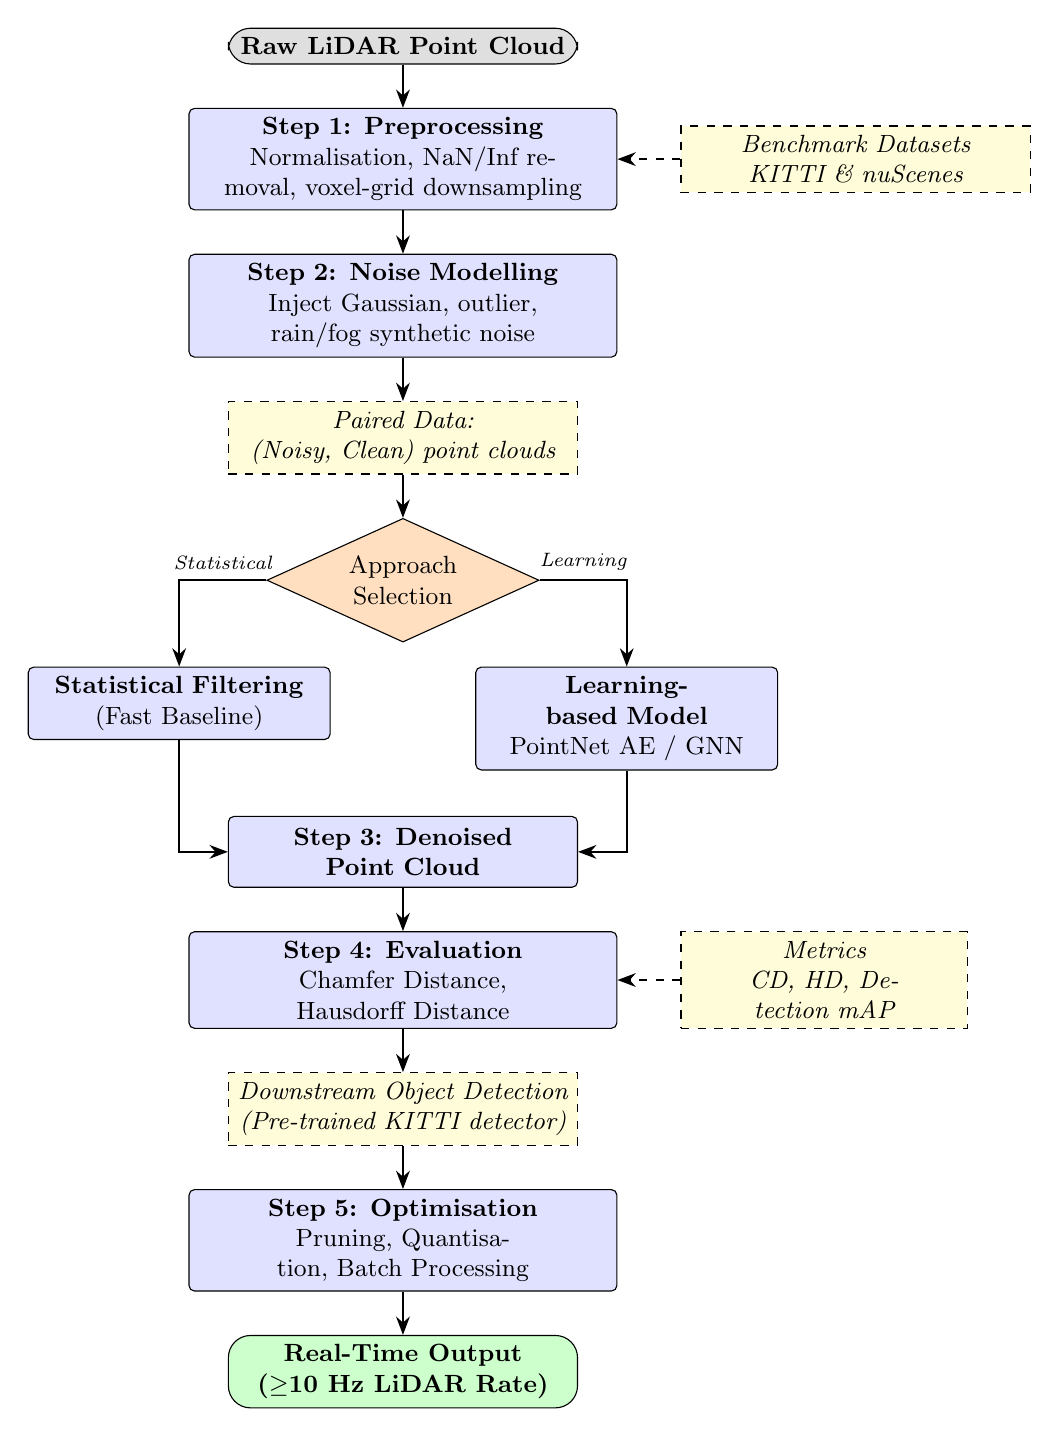
\begin{tikzpicture}[
  node distance=0.55cm,
  box/.style={rectangle, rounded corners=2pt, draw, fill=blue!12,
              text width=5.2cm, align=center, font=\small, minimum height=0.9cm},
  data/.style={rectangle, draw, dashed, fill=yellow!15,
              text width=4.2cm, align=center, font=\small\itshape},
  term/.style={rectangle, rounded corners=8pt, draw, fill=gray!25,
              text width=4.2cm, align=center, font=\small\bfseries},
  outterm/.style={rectangle, rounded corners=8pt, draw, fill=green!20,
              text width=4.2cm, align=center, font=\small\bfseries},
  dec/.style={diamond, aspect=2.2, draw, fill=orange!25, align=center, font=\small},
  arrow/.style={-{Stealth}, thick},
]
\node[term] (raw) {Raw LiDAR Point Cloud};
\node[box, below=of raw] (pre) {\textbf{Step 1: Preprocessing}\\
  Normalisation, NaN/Inf removal, voxel-grid downsampling};
\node[data, right=0.8cm of pre] (bench) {Benchmark Datasets\\KITTI \& nuScenes};
\node[box, below=of pre] (noise) {\textbf{Step 2: Noise Modelling}\\
  Inject Gaussian, outlier, rain/fog synthetic noise};
\node[data, below=of noise] (paired) {Paired Data:\\(Noisy, Clean) point clouds};
\node[dec, below=of paired] (sel) {Approach\\Selection};
\node[box, below left=0.7cm and 0.05cm of sel, text width=3.6cm] (stat)
  {\textbf{Statistical Filtering}\\(Fast Baseline)};
\node[box, below right=0.7cm and 0.05cm of sel, text width=3.6cm] (learn)
  {\textbf{Learning-based Model}\\PointNet AE / GNN};
\node[box, below=2.2cm of sel, text width=4.2cm] (den)
  {\textbf{Step 3: Denoised Point Cloud}};
\node[box, below=of den] (eval) {\textbf{Step 4: Evaluation}\\
  Chamfer Distance, Hausdorff Distance};
\node[data, right=0.8cm of eval, text width=3.4cm] (met) {Metrics\\CD, HD, Detection mAP};
\node[data, below=of eval] (det) {Downstream Object Detection\\(Pre-trained KITTI detector)};
\node[box, below=of det] (opt) {\textbf{Step 5: Optimisation}\\
  Pruning, Quantisation, Batch Processing};
\node[outterm, below=of opt] (out) {Real-Time Output\\($\geq$10 Hz LiDAR Rate)};

\draw[arrow] (raw) -- (pre);
\draw[arrow, dashed] (bench) -- (pre);
\draw[arrow] (pre) -- (noise);
\draw[arrow] (noise) -- (paired);
\draw[arrow] (paired) -- (sel);
\draw[arrow] (sel) -| node[above, font=\scriptsize\itshape, pos=0.25] {Statistical} (stat);
\draw[arrow] (sel) -| node[above, font=\scriptsize\itshape, pos=0.25] {Learning} (learn);
\draw[arrow] (stat) |- (den);
\draw[arrow] (learn) |- (den);
\draw[arrow] (den) -- (eval);
\draw[arrow, dashed] (met) -- (eval);
\draw[arrow] (eval) -- (det);
\draw[arrow] (det) -- (opt);
\draw[arrow] (opt) -- (out);
\end{tikzpicture}}
\captionof{figure}{Logical flow diagram of the proposed LiDAR point cloud
denoising system.}
\label{fig:flow}
\end{center}
\clearpage

The proposed methodology involves a stepwise approach for designing and
evaluating a LiDAR point cloud denoising system.

\begin{description}
\item[Step 1: Dataset Study and Preprocessing]\hfill\\
Benchmark datasets - KITTI \cite{geiger2012kitti} and nuScenes
\cite{caesar2020nuscenes} - will be studied to understand the characteristics
of real-world LiDAR data. Input point clouds will undergo preprocessing steps
such as normalisation, removal of invalid (NaN/Inf) points, and voxel-grid
downsampling to reduce computational overhead.

\item[Step 2: Noise Modelling]\hfill\\
Synthetic noise (Gaussian, random outliers, rain/fog simulation) will be
injected into clean point clouds to create paired (noisy, clean) training
data. This supervised training signal enables quantitative evaluation of
denoising quality.

\item[Step 3: Denoising Pipeline Design]\hfill\\
A denoising technique will be selected and implemented. The approach may
include: (a) statistical filtering as a fast baseline, or (b) a
learning-based model (e.g., PointNet-based autoencoder or lightweight graph
neural network) depending on feasibility. The goal is to remove noise while
preserving the geometric structure of objects in the scene.

\item[Step 4: Evaluation]\hfill\\
Performance will be assessed by comparing original and processed point clouds
using metrics such as Chamfer Distance and Hausdorff Distance. The impact on
downstream object detection accuracy (using a pre-trained detector on KITTI)
will also be measured.

\item[Step 5: Optimisation for Real-Time Performance]\hfill\\
The pipeline will be profiled and optimised (e.g., model pruning,
quantisation, or batch processing) to determine suitability for near
real-time operation, targeting throughput compatible with typical LiDAR scan
rates (10~Hz).
\end{description}
\clearpage

% ═══════════════════════ 6. Project Requirements ═══════════════════════
\section{Project Requirements}

\subsection*{Technical Requirements}
\begin{itemize}
\item \textbf{Programming Language:} Python
\item \textbf{Frameworks:} PyTorch / TensorFlow for model development and training
\item \textbf{Libraries:} Open3D and PCL for point cloud processing; NumPy for
      numerical operations
\item \textbf{Datasets:} KITTI and nuScenes (publicly available LiDAR benchmarks)
\item \textbf{Compute:} GPU access (minimum 8~GB VRAM recommended) for training
      deep learning models
\end{itemize}

\subsection*{Hardware Requirements}
\begin{itemize}
\item \textbf{LiDAR Sensor:} YDLIDAR X2 2D LiDAR sensor for live data collection
      and pipeline testing
\item \textbf{Interface:} USB / Ethernet connection to host machine
\item \textbf{Mount:} Tripod or fixed stand for stable scanning
\item \textbf{Compute Platform:} Laptop or desktop (primary development);
      Raspberry Pi for lightweight embedded inference testing
\end{itemize}
\clearpage

% ═══════════════════════ 7. Work Plan ═══════════════════════
\section{Work Plan}

The project will be executed over a period of six months as outlined in
Table~\ref{tab:workplan} and the Gantt chart in Figure~\ref{fig:gantt}.

\begin{table}[h]
\centering
\caption{Six-month work plan for the capstone project.}
\label{tab:workplan}
\renewcommand{\arraystretch}{1.4}
\begin{tabular}{|c|p{8.2cm}|p{3.2cm}|}
\hline
\textbf{Month} & \textbf{Activity} & \textbf{Milestone}\\\hline
1 & Literature survey and problem understanding & Survey report\\\hline
2 & Dataset study (KITTI, nuScenes) and noise modelling & Dataset ready\\\hline
3 & Selection and initial implementation of denoising technique & Baseline result\\\hline
4 & Design and refinement of complete pipeline & Working pipeline\\\hline
5 & Evaluation, analysis, and optimisation & Evaluation report\\\hline
6 & Documentation and final report preparation & Final report\\\hline
\end{tabular}
\end{table}

\begin{figure}[h]
\centering
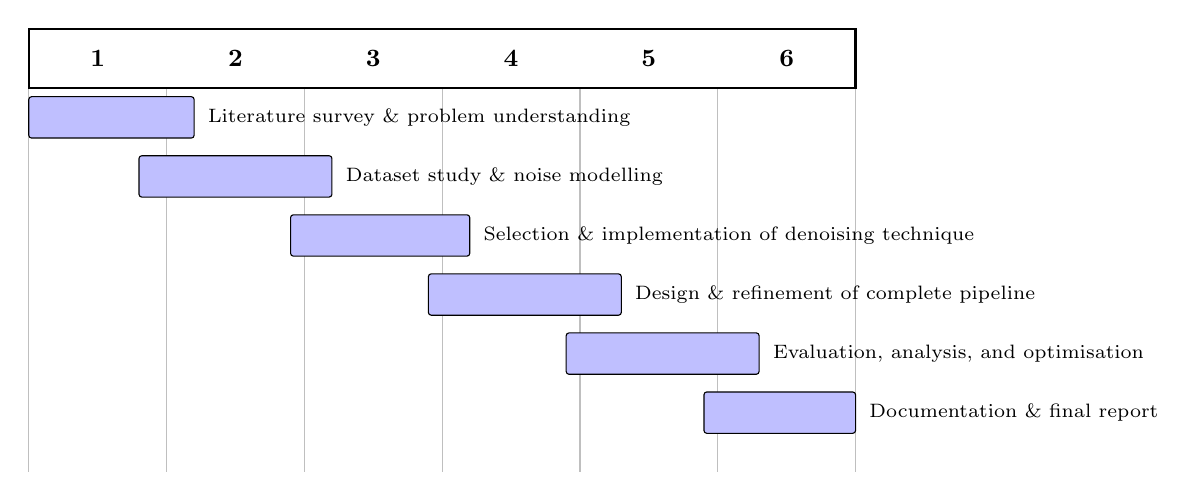
\begin{tikzpicture}[x=1.75cm, y=0.75cm]
% grid and month headers
\foreach \m in {1,...,6} {
  \node[font=\small\bfseries] at (\m - 0.5, 0.5) {\m};
  \draw[gray!50] (\m - 1, 0) -- (\m - 1, -6.5);
}
\draw[gray!50] (6, 0) -- (6, -6.5);
\draw[thick] (0, 0) rectangle (6, 1);
% bars: {start month-1, row, length, label}
\foreach \s/\r/\l/\t in {
  0/1/1.2/{Literature survey \& problem understanding},
  0.8/2/1.4/{Dataset study \& noise modelling},
  1.9/3/1.3/{Selection \& implementation of denoising technique},
  2.9/4/1.4/{Design \& refinement of complete pipeline},
  3.9/5/1.4/{Evaluation, analysis, and optimisation},
  4.9/6/1.1/{Documentation \& final report}} {
  \draw[fill=blue!25, rounded corners=1pt]
    (\s, -\r + 0.15) rectangle (\s + \l, -\r + 0.85);
  \node[right, font=\scriptsize, align=left]
    at (\s + \l + 0.03, -\r + 0.5) {\t};
}
\end{tikzpicture}
\caption{Gantt chart illustrating the six-month project timeline and milestones.}
\label{fig:gantt}
\end{figure}
\clearpage

% ═══════════════════════ 8. Outcomes & Roles ═══════════════════════
\section{Project Outcomes \& Individual Roles}

\subsection*{Expected Outcomes}
\begin{itemize}
\item A well-defined LiDAR point cloud denoising framework (code and
      documentation).
\item Performance comparison of different denoising approaches (statistical
      vs. learning-based).
\item Analysis of the impact of denoising on downstream object detection
      accuracy.
\item Final project report and presentation.
\end{itemize}

\subsection*{Individual Roles}
% TODO(team): Name column intentionally left blank pending confirmation of
% the "Siddant"/"Siddhant" spelling; roll numbers identify each member.
\begin{table}[h]
\centering
\caption{Individual roles and responsibilities.}
\label{tab:roles}
\renewcommand{\arraystretch}{1.5}
\begin{tabular}{|p{4cm}|p{2.6cm}|p{6.4cm}|}
\hline
\textbf{Name} & \textbf{Roll No.} & \textbf{Responsibilities}\\\hline
 & 102315219 & Literature review\\\hline
 & 102303537 & Dataset analysis\\\hline
 & 102303640 & Methodology design and implementation\\\hline
 & 102303703 & Evaluation, benchmarking, and optimisation\\\hline
 & 102315247 & Documentation and report preparation\\\hline
\end{tabular}
\end{table}
\clearpage

% ═══════════════════════ 9. Course Subjects ═══════════════════════
\section{Course Subjects}

The successful execution of this project will require knowledge from the
following subjects:

\begin{itemize}
\item \textbf{Machine Learning} - for understanding and implementing
      learning-based denoising models.
\item \textbf{Computer Vision} - for 3D scene understanding, object detection,
      and point cloud processing.
\item \textbf{Data Structures and Algorithms} - for efficient neighbourhood
      search (k-d tree, octree) and pipeline design.
\item \textbf{Linear Algebra} - for geometric transformations and matrix
      operations on point cloud data.
\item \textbf{Probability and Statistics} - for statistical filtering
      techniques and performance metric analysis.
\item \textbf{Parallel Computing} (\emph{optional}) - for GPU-accelerated
      processing to achieve near real-time performance.
\end{itemize}
\clearpage

% ═══════════════════════ 10. References ═══════════════════════
\section{References}

\begin{thebibliography}{12}

\bibitem{qi2017pointnet}
C.~R. Qi, H.~Su, K.~Mo, and L.~J. Guibas, ``PointNet: Deep Learning on Point
Sets for 3D Classification and Segmentation,'' in \emph{Proc. IEEE/CVF
Conference on Computer Vision and Pattern Recognition (CVPR)}, pp. 652--660,
2017.

\bibitem{qi2017pointnetpp}
C.~R. Qi, L.~Yi, H.~Su, and L.~J. Guibas, ``PointNet++: Deep Hierarchical
Feature Learning on Point Sets in a Metric Space,'' in \emph{Advances in
Neural Information Processing Systems (NeurIPS)}, vol.~30, 2017.

\bibitem{geiger2012kitti}
A.~Geiger, P.~Lenz, and R.~Urtasun, ``Are we ready for autonomous driving?
The KITTI Vision Benchmark Suite,'' in \emph{Proc. IEEE/CVF Conference on
Computer Vision and Pattern Recognition (CVPR)}, pp. 3354--3361, 2012.

\bibitem{caesar2020nuscenes}
H.~Caesar, V.~Bankiti, A.~H. Lang, S.~Vora, V.~E. Liong, Q.~Xu, A.~Krishnan,
Y.~Pan, G.~Baldan, and O.~Beijbom, ``nuScenes: A Multimodal Dataset for
Autonomous Driving,'' in \emph{Proc. IEEE/CVF Conference on Computer Vision
and Pattern Recognition (CVPR)}, pp. 11621--11631, 2020.

\bibitem{wang2025survey}
J.~Wang, B.~Fei, D.~de Silva Edirimuni, Z.~Liu, Y.~He, and X.~Lu, ``A Survey
of Deep Learning-based Point Cloud Denoising,'' \emph{arXiv preprint},
arXiv:2508.17011, 2025.

\bibitem{heinzler2020cnn}
R.~Heinzler, P.~Schindler, J.~Seekircher, W.~Ritter, and W.~Stork,
``CNN-based LiDAR Point Cloud De-Noising in Adverse Weather,'' \emph{IEEE
Robotics and Automation Letters}, vol.~5, no.~2, pp. 2514--2521, 2020.

\bibitem{rusu2011pcl}
R.~B. Rusu and S.~Cousins, ``3D is here: Point Cloud Library (PCL),'' in
\emph{Proc. IEEE International Conference on Robotics and Automation (ICRA)},
pp. 1--4, 2011.

\bibitem{wang2019dgcnn}
Y.~Wang, Y.~Sun, Z.~Liu, S.~E. Sarma, M.~M. Bronstein, and J.~M. Solomon,
``Dynamic Graph CNN for Learning on Point Clouds,'' \emph{ACM Transactions on
Graphics}, vol.~38, no.~5, pp. 1--12, 2019.

\bibitem{zhao2021point}
H.~Zhao, L.~Jiang, J.~Jia, P.~Torr, and V.~Koltun, ``Point Transformer,'' in
\emph{Proc. IEEE/CVF International Conference on Computer Vision (ICCV)},
pp. 16259--16268, 2021.

\bibitem{ho2020ddpm}
J.~Ho, A.~Jain, and P.~Abbeel, ``Denoising Diffusion Probabilistic Models,''
in \emph{Advances in Neural Information Processing Systems (NeurIPS)},
vol.~33, pp. 6840--6851, 2020.

\bibitem{cao2019adversarial}
Y.~Cao, C.~Xiao, B.~Cyr, Y.~Zhou, W.~Park, S.~Rampazzi, Q.~A. Chen, K.~Fu,
and Z.~M. Mao, ``Adversarial Sensor Attack on LiDAR-based Perception in
Autonomous Driving,'' in \emph{Proc. ACM SIGSAC Conference on Computer and
Communications Security (CCS)}, pp. 2267--2281, 2019.

\bibitem{sun2020towards}
J.~Sun, Y.~Cao, Q.~A. Chen, and Z.~M. Mao, ``Towards Robust LiDAR-based
Perception in Autonomous Driving: General Black-box Adversarial Sensor Attack
and Countermeasures,'' in \emph{Proc. 29th USENIX Security Symposium},
pp. 877--894, 2020.

\end{thebibliography}
\clearpage

\end{document}
